%=========================================================================
% sec-intro
%=========================================================================

\section{Introduction}
\label{sec-intro}

%=========================================================================
% fig-intro-dgemm.tex
%=========================================================================

\begin{figure}[h]

  \centering
  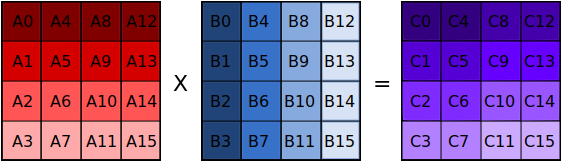
\includegraphics[width=0.7\tw]{fig-intro-dgemm.svg.pdf}

  \caption{\textbf{Double-Precision General Matrix-Matrix Multiply --}
    For simplicity, 4x4 matrices are shown with elements labeled in the
    column-major order. Rows of input matrix {\tt{A}} is multiplied with
    columns of input matrix {\tt{B}} and accumulated to generate the
    output matrix {\tt{C}}.}

  \label{fig-intro-dgemm}

\end{figure}


In this report, we explore several optimizations for improving the
performance of double-precision general matrix-matrix multiply
(DGEMM). The DGEMM algorithm, as shown in Figure~\ref{fig-intro-dgemm},
is a standard matrix multiplication between two input matrices with
double-precision floating point elements to generate an output
matrix. The serial algorithm computes elements of the output matrix
{\tt{C}} from input matrices {\tt{A}} and {\tt{B}} as follows:

\[
C_{ij} = \sum_{k=0}^{N}A_{ik}*B_{kj}
\]
\smallskip

We use a standard blocking algorithm that computes smaller pieces of the
output matrices at a time as a baseline for our optimizations. The
high-level goals of the optimizations are to improve the code generated
by the compiler, maximize hardware resource utilization, and produce more
desirable memory access patterns.
\smallskip

